\appendix

\setcounter{page}{1}
\renewcommand\thefigure{\thesection\arabic{figure}}
\setcounter{figure}{0} 

\onecolumngrid

\begin{center}
\large{ Supplementary Material for \\ ``Deep Circuit Compression for Quantum Dynamics via Tensor Networks''
}
\end{center}

\section{Hamiltonians}\label{sec:Hamiltonians}

Here we further detail the Hamiltonians studied in our numerical results in Sec.~\ref{sec:results}.

\begin{figure*}[b!]
\centering
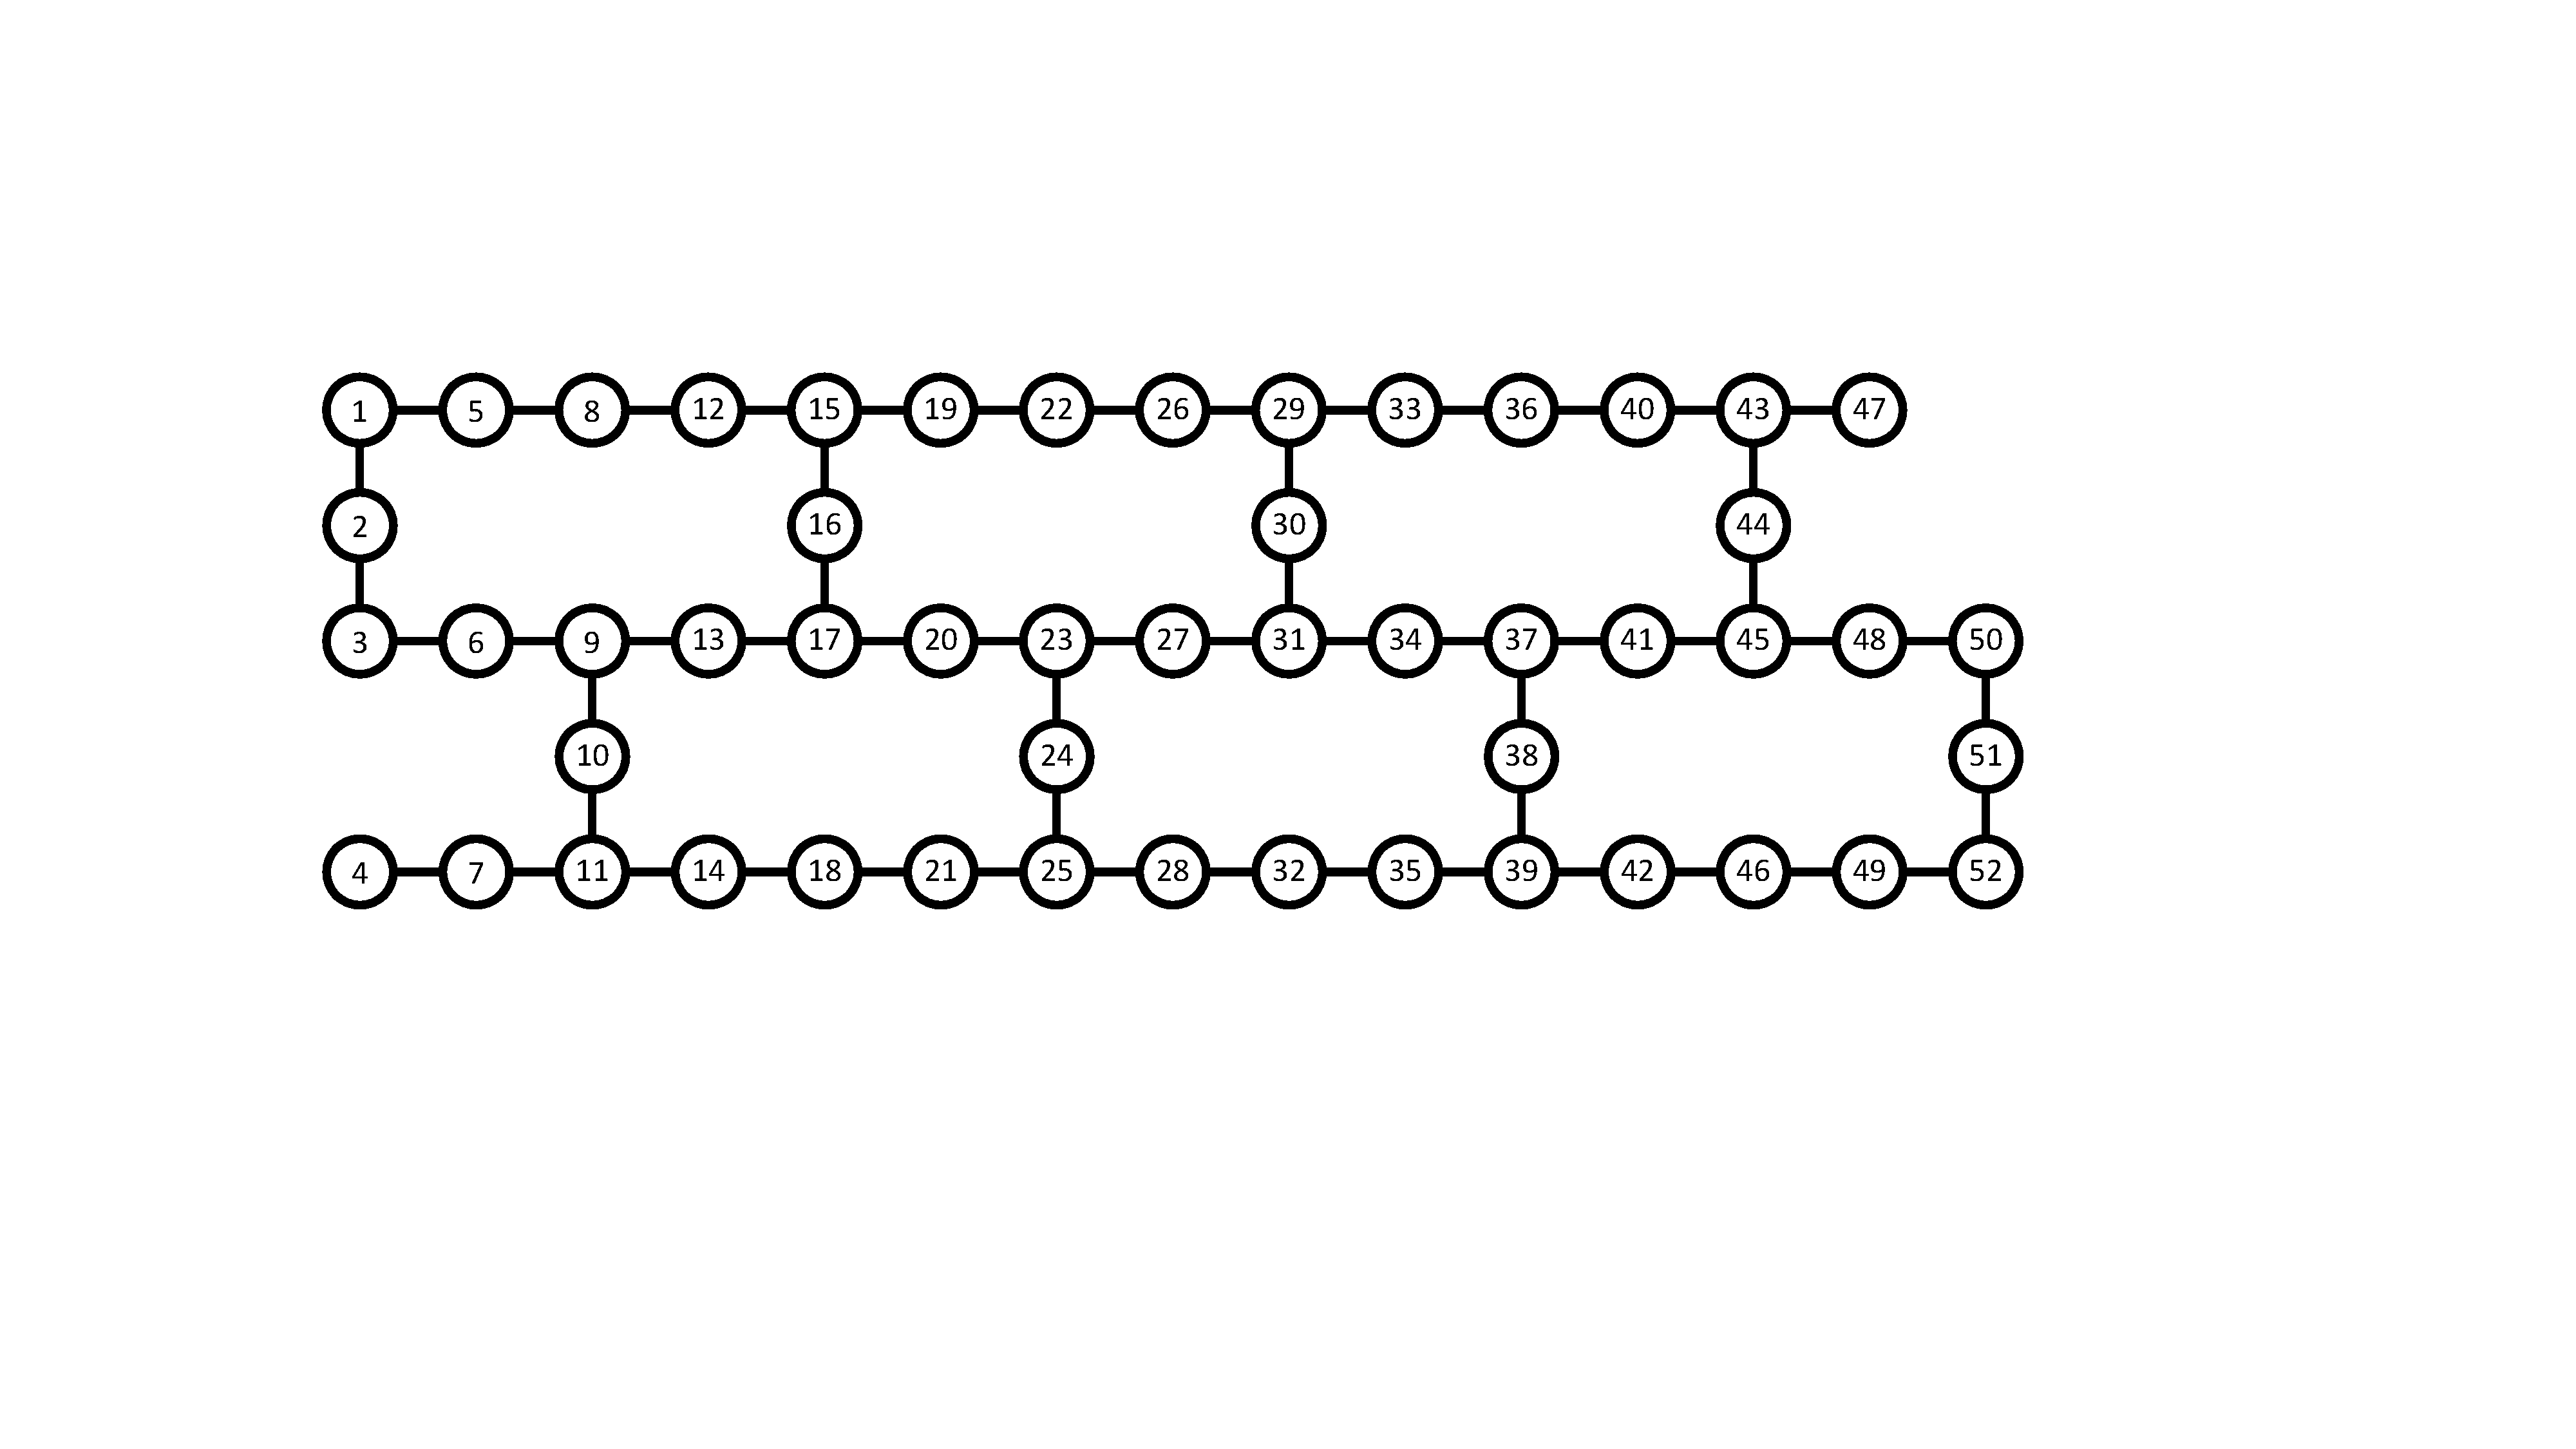
\includegraphics[width=0.9\textwidth]{figures/MPOCompFigures_HeavyHex.pdf}
\vspace{-2mm}
\caption{\textbf{Heavy Hex Topology. }For the 2D compilation demonstration, the Hamiltonian chosen is the Transverse-Field Ising model with the same connectivity graph as the shown 52 qubit subset of the IBM Heavy-Hex topology. To map the local 2D gates onto the MPO, we use a winding across the shortest dimension, as indicated by the qubit numbering.}
\label{fig:HeavyHex}
\vspace{-1.5em}
\end{figure*}


\textbf{1) 1D Transverse-Field Ising model}

\begin{equation}
    H = \sum_{i=1}^{n-1} Z_i Z_{i+1} + h\sum_{i=1}^n X_i
\end{equation}

We target a 200 qubit chain, with a field strength of $h=1.0$ for a total evolution time of $t=2.0$.

\bigskip

\textbf{2) 1D Hubbard model}

\begin{equation}
\begin{split}
    H = -t_{\text{hop}}\sum_{i,\sigma} \left( c^{\dagger}_{i,\sigma}c_{i+1,\sigma} + c^{\dagger}_{i+1,\sigma}c_{i,\sigma} \right) + U\sum_{i} n_{i,\uparrow}n_{i,\downarrow}
\end{split}
\end{equation}

We use a staggered representation where the spin up/down orbitals are neighboring on a 1D chain. We target the Hamiltonian with 50 sites (corresponding to 100 qubits), with $U=4.0$, $t_{\text{hop}}=1.0$, and total evolution time $t=0.2$. We assume access to a 1D chain of qubits with nearest-neighbor interactions; the next-nearest neighbor interaction for the hopping terms therefore requires fermionic SWAP gates in the Trotter unitaries.

\bigskip

\textbf{3) 1D $J_1-J_2$ Model}

\begin{equation}
\begin{split}
    H = J_1\sum_{i=1}^{n-1} \bar{\sigma}_i \cdot \bar{\sigma}_{i+1} + J_2\sum_{i=1}^{n-2} \bar{\sigma}_i \cdot \bar{\sigma}_{i+2} 
\end{split}
\end{equation}

We target a chain of 40 qubits for a total evolution time of $t=1.0$, with $J_1=1.0$ and $J_2 = 0.25$.
We assume access to a 1D chain of qubits with nearest-neighbor interactions; the next-nearest neighbor interaction therefore requires SWAP gates in the Trotter unitaries.

\bigskip

\textbf{4) Transverse-Field Ising model on the Heavy Hex topology}

We also compile circuits for the Transverse-Field Ising model on the 2D Heavy-Hex topology found on IBM superconducting chips. For the 2D compilation, we compile the circuit directly onto the same topology, generating a circuit that has the same local 2D interactions as the real quantum device. We target the 52 qubit subset of qubits shown in Fig.~\ref{fig:HeavyHex}. We set $h=0.75$, and $t=0.5$.

\clearpage